\documentclass[11pt]{article}
\usepackage[utf8]{inputenc}
\usepackage{lmodern}
\usepackage[english]{babel}
\usepackage{blindtext}
\usepackage[a4paper,top=2cm,bottom=2cm,left=3cm,right=3cm,marginparwidth=1.75cm]{geometry}
\renewcommand{\familydefault}{\sfdefault}
\usepackage{amsmath}
\usepackage{graphicx}
\usepackage[colorlinks=true, allcolors=blue]{hyperref}

\setcounter{secnumdepth}{4}
\usepackage{titlesec}

\usepackage[skip=6pt]{parskip}

\usepackage[backend=biber, style=ieee, sorting=none]{biblatex}
\addbibresource{bibliography.bib}
\usepackage[shortlabels]{enumitem}
\usepackage[table,xcdraw]{xcolor}
\usepackage{hyperref}
\hypersetup{colorlinks=true, allcolors=blue}
\usepackage[nameinlink,noabbrev,capitalize]{cleveref}
\usepackage{colortbl}
\usepackage[section]{placeins}
\usepackage{subcaption}
\usepackage{longtable}
\usepackage{comment}
\usepackage{caption}
\captionsetup{font=footnotesize}
\setlength{\parindent}{0pt}
\usepackage{titlesec}
\titlespacing*{\section} {0pt}{3ex}{2ex}
\titlespacing*{\subsection} {0pt}{3ex}{2ex}
\titlespacing*{\subsubsection} {0pt}{3ex}{2ex}
\usepackage{pdfpages}
\setlist{nolistsep,leftmargin=*}

\usepackage{tocloft}
\setlength{\cftsecindent}{0pt}
\setlength{\cftsubsecindent}{1.2em}
\setlength{\cftsecnumwidth}{2.2em}
\setlength{\cftsubsecnumwidth}{3.0em}
\setcounter{tocdepth}{2}

\titleformat{\paragraph}
{\normalfont\normalsize\bfseries}
{}
{0pt}
{}

\usepackage{booktabs}

\usepackage{float}
\usepackage{tabularx}
\usepackage{wrapfig}

\title{Maintenance and Troubleshooting\\[0.3em]
\large COM2020 - Project 7}
\author{Emre Acarsoy, Luca Croci, Tom Croft, Will Finney, Kazybek Khairulla, Luca Pacitti, \\ Harry Taylor}
\date{\today}
\begin{document}
\maketitle
\tableofcontents
\newpage
\section{Overview}
In this document we will outline the information needed to undergo routine maintenance operations for the project. We will then provide detailed troubleshooting instructions, stating possible symptoms of different problems, solutions, and verification methods to ensure problems are resolved. Lastly we will provide a detailed architecture schema followed by steps for routine application extensions.

\section{Maintenance}
\subsection{Clearing Telemetry Data}
Telemetry data can be cleared from within the telemetry app. This is done by opening the app, logging in, and using the "clear telemetry data" function. Detailed instructions are available in the deployment and operations guide.
\subsection{Clearing Logs}
Logs can be cleared by simply deleting them, or their contents. Authentication logs are located in \verb|telemetry/auth/logs.txt|.
\subsection{Backups}
The system does not feature explicit backup mechanisms, thus any backup mechanisms may be used. The data management guide provides details about every data store and its format, which may help in determining a backup mechanism. It should be noted all data stores are plaintext. 

\subsection{Naming Conventions}
The Java application uses pascal case for all classes, interfaces and enum names. It uses camel case for all fields and methods. It uses screaming snake case for constants. All interfaces have the word "Interface" appended to their name. All enums have the word "Enum" appended to their name. All singleton classes have "Singleton" appended to their name. All exceptions have "Exception" appended to their name. All upgrades have "Upgrade" appended to their name. All attack ability granting upgrades follow the convention <Attack Ability Name>UnlockUpgrade. All telemetry events have "Event" appended to their name. Each java file is named after the class it holds.

The Python application uses snake case for all methods and fields, and uses pascal case for classes. It uses screaming snake case for constants, and classes containing only constants are also named in screaming snake case. Files are named in snake case.
\section{Troubleshooting}

\subsection{Cannot Launch Python Application}
\subsubsection{Symptoms}
\begin{itemize}
  \item Get an error: \verb|ModuleNotFoundError: No module named '<Module>'|
  \item Get an error: \verb|python : The term 'python' is not recognized as ...|\\ or \verb|python3 : The term 'python3' is not recognized as ...|
  \item Get an error: \verb|Command 'python3' not found, did you mean: ...|

\end{itemize}
\subsubsection{Solutions}
Try each of these solutions, and verify if it worked before trying the next.
\begin{enumerate}
  \item Ensure you're using a supported operating system (Linux, Windows or macOS)
  \item Follow the prerequisite installation and deployment instructions detailed in the deployment and operations guide. 
  \item Uninstall all prerequisites and go through all the steps for prerequisite installation and app deployment. 
\end{enumerate}

\subsubsection{Verification}
The Python application launches with no errors. 

\subsection{Cannot Launch Java Application}
\subsubsection{Symptoms}
\begin{itemize}
  \item Get an error: \verb|mvn : The term 'mvn' is not recognized as ...|
  \item Get an error: \verb|Command 'mvn' not found, did you mean: ..|
  \item Get an error: \\\verb|The JAVA_HOME environment variable is not defined correctly ...|
\end{itemize}
\subsubsection{Solutions}
Try each of these solutions, and verify if it worked before trying the next.
\begin{enumerate}
  \item Ensure you're using a supported operating system (Linux, Windows or macOS)
  \item Follow the prerequisite installation and deployment instructions detailed in the deployment and operations guide. 
  \item Uninstall all prerequisites and go through all the steps for prerequisite installation and app deployment. 
\end{enumerate}

\subsubsection{Verification}
The Java application launches with no errors. 

\subsection{Cannot Log In}
\subsubsection{Symptoms}
\begin{itemize}
  \item Java application displays something like \ref{fig:java_login_fail}.
  \item Python application displays something like \ref{fig:python_login_fail}.
    \item Error in terminal appears: \verb|Failed to resolve 'accounts.google.com'|
    \item Error in terminal appears:\\\verb|RuntimeError: Could not parse user roles file at logins_file.json- invalid json.|
    \item Error in terminal appear: \\ \verb|ValueError: Logins file at logins_file.jsoncontained an unknown role|
\end{itemize}

\begin{figure}[H]
  \centering
  \begin{minipage}{0.48\textwidth}
    \centering
    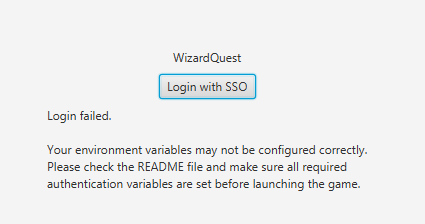
\includegraphics[width=\linewidth]{images/java_login_fail.png}
    \caption{Error causes Java application to be unable to authenticate user.}
    \label{fig:java_login_fail}
  \end{minipage}
  \hfill
  \begin{minipage}{0.48\textwidth}
    \centering
    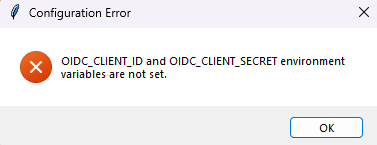
\includegraphics[width=\linewidth]{images/python_login_fail.png}
    \caption{Error causes Python application to be unable to authenticate user.}
    \label{fig:python_login_fail}
  \end{minipage}
\end{figure}

\subsubsection{Solutions}
For each solution, check if it worked using the verification steps before attempting the next.
\begin{enumerate}
  \item Set environment variables, as described in the deployment and operations guide.
  \item Ensure a web browser is installed
  \item Ensure you have internet access
    \item Ensure \verb|logins_file.json| is syntactically valid using \href{https://jsonformatter.org/}{this}.
    \item Ensure that all roles in \verb|logins_file.json| are the correct domain described in the data management guide.
\end{enumerate}

\subsubsection{Verification}
The issue is fixed if \verb|logins_file.json| is syntactically correct, and you can log in on the desired application.

\subsection{Syntax Errors in Telemetry Store}
\subsubsection{Symptoms}
\begin{itemize}
  \item Dashboard views are blank like \ref{fig:blank_dashboards}.
  \item Dashboard views don't update.
    \item A runtime error appears in the terminal \\\verb|RuntimeError: Could not parse - invalid json.|
\end{itemize}

\begin{figure}[H]
  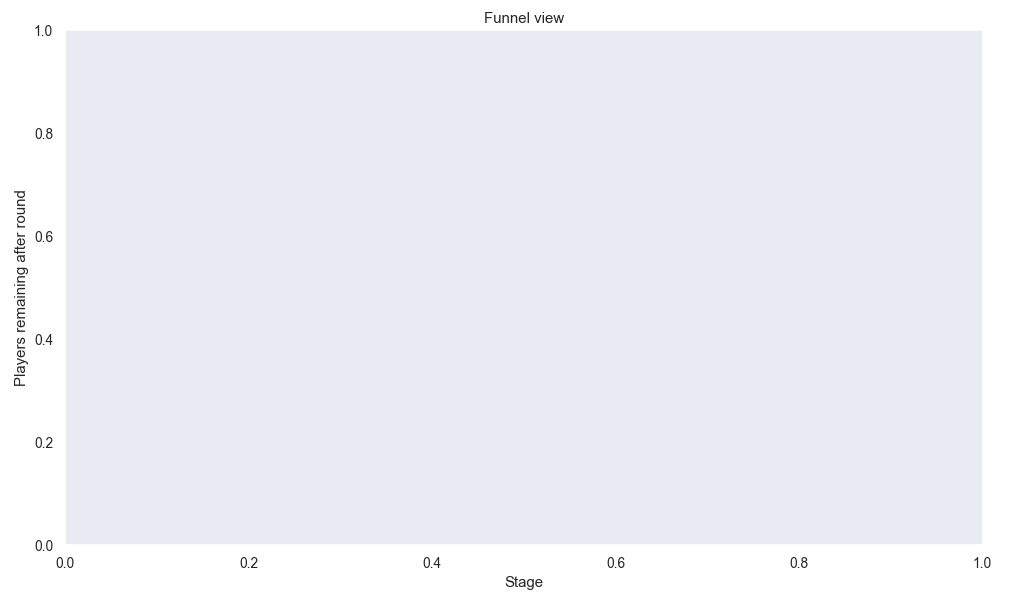
\includegraphics[width=\linewidth]{images/blank_dashboards.png}
  \caption{Error causes dashboards to display blank}
  \label{fig:blank_dashboards}
\end{figure}
\subsubsection{Solutions}
First find which event store(s) has syntax errors. This can be done by going through the following steps on both event stores.
\begin{enumerate}
  \item Check the file is not empty.
    \item Check the file starts with \verb|[| and ends with \verb|]|.
  \item Check between each JSON object is a comma.
  \item Place the JSON file into an online JSON validator such as \href{https://jsonformatter.org/}{this}. If it says it's invalid this file has a syntax error.
\end{enumerate}

Then, correct the syntax error by trying each of the following steps, then using the verification steps to see if it has resolved the problem. If the previous step does not work, try the next.
\begin{enumerate}
  \item Correct the syntax error manually, by for example adding a comma.
  \item Removing the object with the syntax error.
  \item Deleting the telemetry event store.
  \item Deleting both telemetry event stores.
\end{enumerate}
\subsubsection{Verification}
To verify the problem is resolved, first place the JSON store in an online \href{https://jsonformatter.org/}{validator}. If the validator says it is valid, next test that none of the symptoms observed appear in either application after restarting them. If no symptoms persist the issue is resolved.

\section{Architecture}
\subsection{Overview}
The project is split into two applications, one written in Python and the other written in Java. The Python application is in charge of reading telemetry data, interpreting this information, and displaying this to the user. The Java application is in charge of managing user roles, settings, and achievements, design parameters, telemetry generation, and gameplay. 

Both applications communicate via several data stores detailed in the data management guide. Individual methods and fields are not listed, as those are available in the documentation either via pydoc or javadoc. 
\subsection{Python Application}
\subsubsection{Overview}
The Python application is split into 3 sub-modules. Auth handles user authentication through Google OAuth, and provides a wrapper for interfacing with the Java application. Core handles data ingestion, and interpretation. GUI handles the display and refreshing of telemetry data. 

The app entry point is \verb|telemetry_app.py| which instantiates the GUI and starts the main loop within it.
\subsubsection{auth}
\paragraph{auth\_logger}
This component writes authentication events to the authentication log. This event writing is called by auth.
\paragraph{auth\_wrapper}
This component is called by the Java application to authenticate users. It wraps this information in a JSON string and outputs it to standard out. 
\paragraph{auth}
This component handles authenticating the user, creating a new user account for new users, and getting user roles. 
\subsubsection{core}
\paragraph{events}
This component contains all enums for each enumerated field within telemetry events. It also contains a dataclass for each telemetry event, containing all their fields. 
\paragraph{logic}
This component interprets data passed into it, providing metrics used by the GUI for display, getters for obtaining all events of a given type, and methods to classify ingested data.
\paragraph{parsing}
This component ingests data from the telemetry stores, and returns the event as a dataclass described in events. 
\subsubsection{gui}
\paragraph{gui}
GUI creates the majority of the user interface, creating the window tabs, the decision log, suggestions, and the home page. It also handles button presses and propagates those to the backend. It also refreshes the graphs every three seconds. 
\paragraph{plotting}
Plotting is in charge of generating and displaying all dashboard views of the telemetry, it calls the logic to interpret the telemetry data, and displays this data using matplotlib. 
\subsection{Python Tests}
\subsubsection{Overview}
The testing architecture consists of a unit testing folder, and a resources folder for testing data. 
\subsubsection{unit}
\paragraph{test\_logic}
This component, tests the logic component of the Python application.
\paragraph{test\_parsing}
This component, tests the parsing component of the python application. 
\subsection{Java Application}
\subsubsection{Overview}
The Java application is split into several submodules, each handling a different aspect of the system. The abilities module contains all purchasable abilities (called upgrades internally) for the game, as well as the logic for using attack abilities (internally called abilities). Auth makes authentication requests to the Python application and returns the result in a Java-friendly manner for use in other systems. The entity module contains all entities including the player, along with their AI and interfaces. The gamemanger module contains the code for the game manager, which runs the game, and game run which maintains and contains code for a single run of the game. Telemetry stores all telemetry events and the telemetry listener, and ui stores the code for running and displaying the graphical user interface. 
%TODO now write the paragraphs 
\subsubsection{abilities}
\paragraph{UpgradeBase}
\paragraph{UpgradeEnum}
\paragraph{AbilityEnum}
\paragraph{AttackAbilityUnlockUpgrade}
\paragraph{DamageEnum}
\paragraph{ImprovedDamageUpgrade}
\paragraph{DamageResistanceUpgrade}
\subsubsection{auth}
\paragraph{AuthenticationException}
\paragraph{AuthenticationResult}
\paragraph{AuthenticatorInterface}
\paragraph{Authenticator}
\paragraph{RoleEnum}
\subsubsection{entitiy}
\paragraph{EnemyInterface}
\paragraph{EnemyBase}
\paragraph{ConcreteEnemy}
\paragraph{PlayerInterface}
\paragraph{Player}
\paragraph{EntityAIInterface}
\paragraph{EntityAISingleton}
\paragraph{EntityEnum}
\subsubsection{gamemanger}
\paragraph{LackingResourceException}
\paragraph{Encounter}
\paragraph{EncounterInterface}
\paragraph{EncounterEnum}
\paragraph{GameManger}
\paragraph{GameMangerInterface}
\paragraph{GameRun}
\paragraph{GameRunterface}
\paragraph{TimeManagerInterface}
\paragraph{TimeManagerSingleton}
\subsubsection{settings}
\paragraph{DifficultyEnum}
\paragraph{SettingsEnum}
\paragraph{SettingsInterface}
\paragraph{SettingsSingleton}
\subsubsection{telemmetry}
\paragraph{TelemetryEvent}
\paragraph{SessionEvent}
\paragraph{EncounterEvent}
\paragraph{EncounterCompleteEvent}
\paragraph{EncounterFailEvent}
\paragraph{ConcreteTelemetryEvent}
\paragraph{SessionValidationException}
\paragraph{TimestampValidationException}
\paragraph{UserValidationException}
\paragraph{TelemetryListenerInterface}
\paragraph{TelemetryListenerSingleton}
\subsubsection{ui}
\paragraph{GameRunPage}
\paragraph{SettingsPage}
\paragraph{ShopPage}
\subsection{Java Tests}
\subsubsection{Overview}
The tests are split up into integration and unit tests. From there each test type is split by the module it contains tests for. For ease of reading both unit and integration tests are included for each module's test description 
\subsubsection{abilities}
\paragraph{AbilityEnumUnitTests}
\paragraph{UpgradeUnitTests}
\paragraph{AbilityEnumIntegrationTests}
\subsubsection{entity}
\paragraph{EnemyUnitTests}
\paragraph{PlayerUnitTests}
\paragraph{RandomEntityAIUnitTests}
\paragraph{EntityEnumIntegrationTests}
\subsubsection{telemetry}
\paragraph{TelemetryListenerUnitTests}
\paragraph{TelemetryListenerIntegrationTests}
\section{Extension}

\end{document}
